\hypertarget{dislocationSource_8cpp}{\section{dislocation\-Source.\-cpp File Reference}
\label{d8/d5c/dislocationSource_8cpp}\index{dislocation\-Source.\-cpp@{dislocation\-Source.\-cpp}}
}


Definition of the member functions of the \hyperlink{classDislocationSource}{Dislocation\-Source} class.  


{\ttfamily \#include \char`\"{}dislocation\-Source.\-h\char`\"{}}\\*
Include dependency graph for dislocation\-Source.\-cpp\-:\nopagebreak
\begin{figure}[H]
\begin{center}
\leavevmode
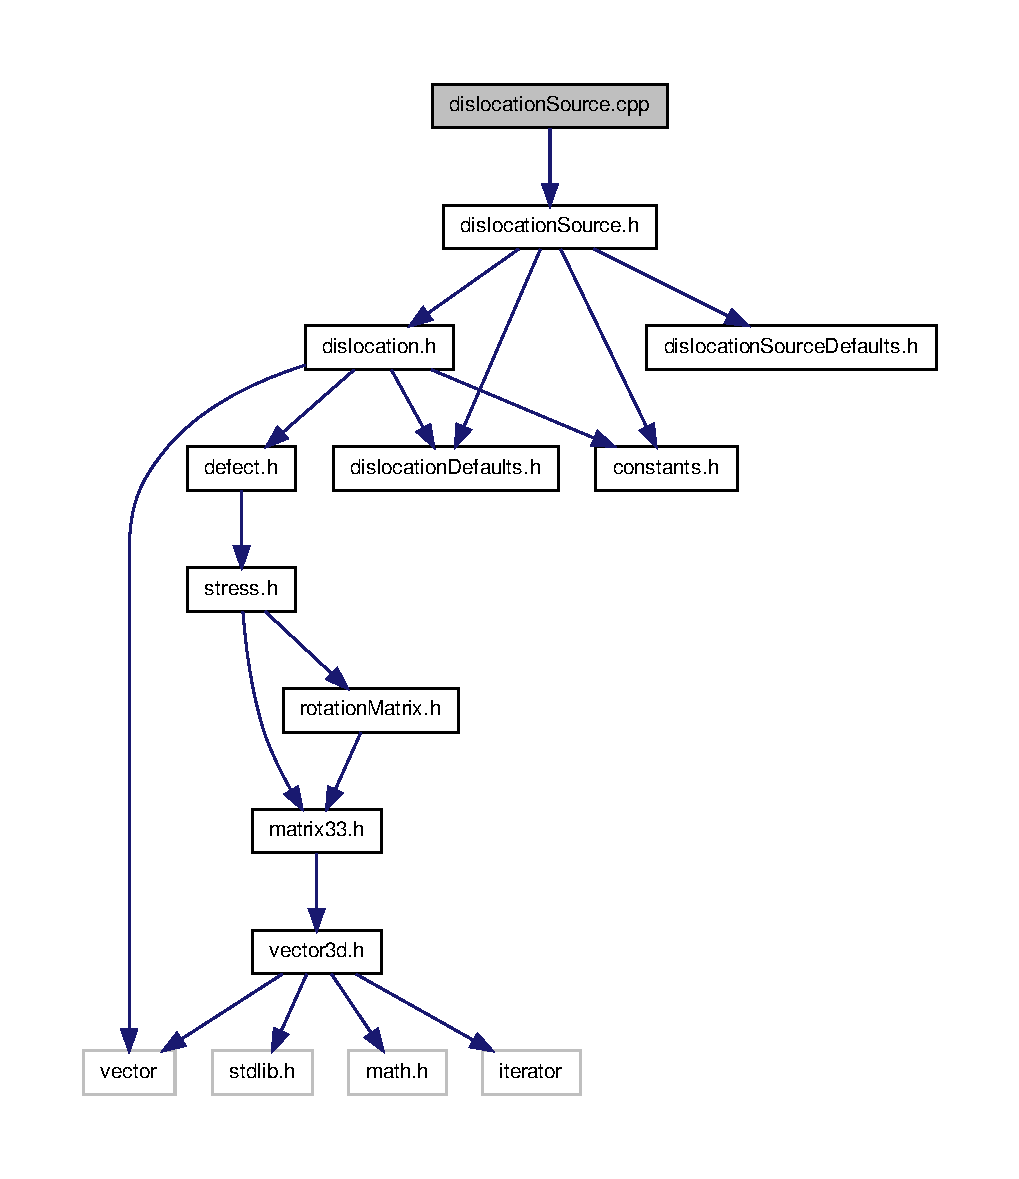
\includegraphics[width=350pt]{df/dbd/dislocationSource_8cpp__incl}
\end{center}
\end{figure}


\subsection{Detailed Description}
Definition of the member functions of the \hyperlink{classDislocationSource}{Dislocation\-Source} class. \begin{DoxyAuthor}{Author}
Adhish Majumdar 
\end{DoxyAuthor}
\begin{DoxyVersion}{Version}
0.\-0 
\end{DoxyVersion}
\begin{DoxyDate}{Date}
05/06/2013
\end{DoxyDate}
This file defines the member functions of the \hyperlink{classDislocationSource}{Dislocation\-Source} class representing a source of dislocations in the simulation. This class inherits from the \hyperlink{classDefect}{Defect} class. This object is basically the representation of a Frank-\/\-Read source emitting dislocation dipoles. When the dislocation source experiences a shear stress greater than a critical value for a certain amount of time (or number of iterations), it emits a dislocation dipole with a length that is a function of the applied stress. 

Definition in file \hyperlink{dislocationSource_8cpp_source}{dislocation\-Source.\-cpp}.

